\chapter{Pixel detector upgrades for \RunTwo}
\label{chap:trackingupgrades}
%
The large event rate expected during \RunTwo\ data taking comes with a significant increase of pile-up events. The separation of pile-up from the hard scatter under study crucially relies on the performance of the tracking system. Furthermore, precise tracking information about charged particles allows for the reconstruction of secondary vertices within jets via the measurement of the spatial distance of the jet origin from the primary vertex. This is the basis for the detection of long-lived particles like \bhadron{s} and the identification of jets originating from a \bquark, referred to as \btag. The \btag\ is vital for \tquark\ mass measurements. Consequently, maintaining or even improving the tracking capabilities of the pixel detector for the harsh environments of \RunTwo\ was a primary goal for the upgrade period during \gls{LS1}.

In the following, the improvements of the \gls{ATLAS} pixel detector system during \gls{LS1} are described, including the results of a year of hardware work at \gls{CERN}. Further information on \gls{ATLAS} upgrade activities can be found in \reference~\cite{CERN-LHCC-2011-012}.







\section{Technical details of the pixel detector and IBL}
The \gls{ATLAS} pixel detector~\cite{pixeltdr} consists of three layers of barrel pixel detectors at radii of 5, 9 and 12~cm from the beam axis, referred to as \blayer, \layerone\ and \layertwo, respectively. With the two end caps of three pixel disks each, the pixel detector carries 1744 pixel modules in total and forms a three-hit system up to a pseudorapidity of $\abseta=2.5$. The modules are mounted on carbon fibre support structures, referred to as staves, which also carry the pipes of the evaporative C$_3$F$_8$ cooling system. This allows for low operation temperatures to counteract the increase of leakage current due to the inevitable radiation damage. The layout of the pixel detector is shown in \fig~\subref*{sfig:pixellayout}. This structure is referred to as the active volume.
%
%%%%%%%%%%%%%%%%%%%%%%%%%%%%%%%%%%%%%%%%%%%%%%%%%%%%%%%%%%%%%%%%%%%%%%%%%%%%%%%
\begin{figure*}[tbp!]
\centering
% 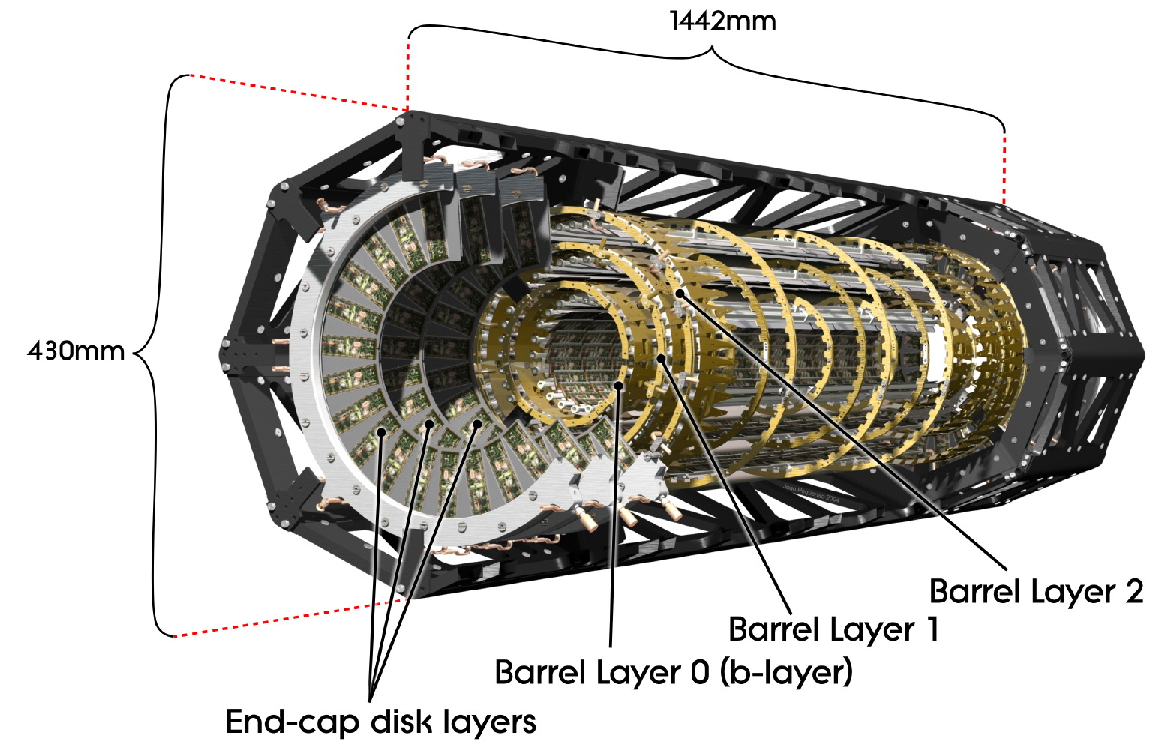
\includegraphics[width=0.8\textwidth]{./figs/PixelPerspective.png}
\subfloat[Structure of the pixel detector]{
  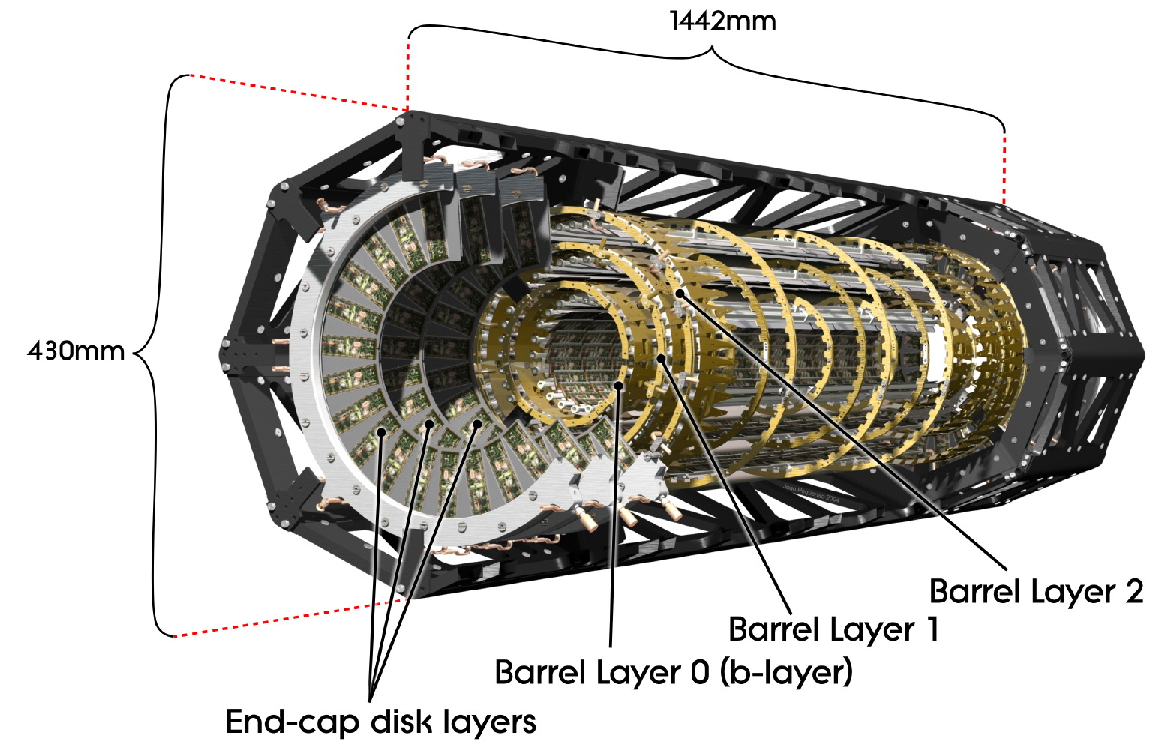
\includegraphics[height=0.4\textwidth]{./figs/PixelPerspective.png}
  \label{sfig:pixellayout}
}
\subfloat[Layout of a pixel module]{
  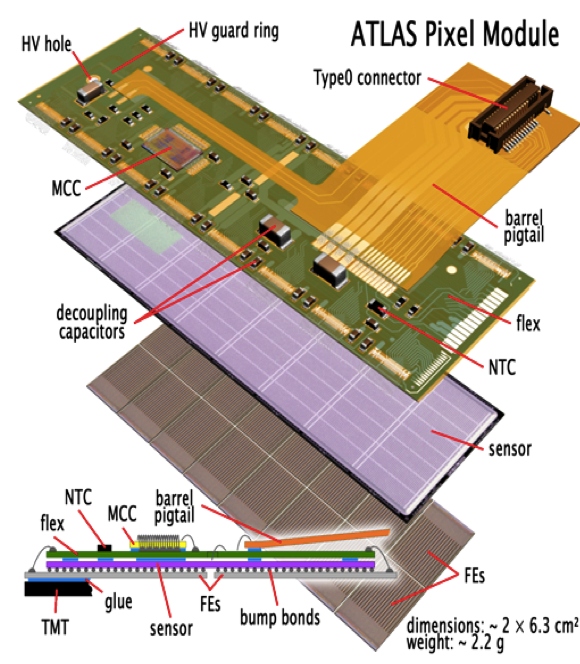
\includegraphics[height=0.4\textwidth]{./figs/ATLAS_pixel_module.png}
  \label{sfig:pixelmodule}
}
\hfill
\caption[The pixel detector and module layout]{
%
\Fig~\subref{sfig:pixellayout} shows a cut through the active volume of the pixel detector during \RunOne, consisting of three disks on each side and three barrel layers of pixel modules. The carbon fiber support structure and the C$_3$F$_8$ cooling pipes are also visible~\cite{ATLASpublic}.
%
\Fig~\subref{sfig:pixelmodule} shows the layout of a typical barrel pixel module~\cite{atlasexp}. 
%
}
\label{fig:Pixellayout}
\end{figure*}
%%%%%%%%%%%%%%%%%%%%%%%%%%%%%%%%%%%%%%%%%%%%%%%%%%%%%%%%%%%%%%%%%%%%%%%%%%%%%%%
%
The pixel modules, shown in \fig~\subref*{sfig:pixelmodule}, consist of a 250~\mum\ thick n-in-n silicon sensor with  $400\times50~\mum^2$ pixels, bump-bonded to 16 \gls{FE} readout chips, and a module flex. The module flex is a printed circuit board made from a thin flexible kapton substrate. It is connected with wire bonds to the \gls{FE} chips and carries the \gls{MCC} and a \gls{NTC} for temperature measurement. Uniform temperature regulation across the module is ensured by the thermal coupling to the coolant provided by the \gls{TMT}. The \gls{FE} chips provide \gls{ToT} values, which can be converted via an approximately linear relation to the amount of deposited charge. 
%
The \gls{MCC} receives the trigger signal and initiates the event data readout from the \gls{FE} chips. The sensors and the electronics are designed to work up to a dose of $1\times10^{15}~$\neqcm, with \neqcm\ being the equivalent dose from neutron radiation.
%
The cooling and electrical \gls{LV} and \gls{HV} are routed from the outside of the detector over about 3.5~m to the active volume via \gls{SQP}, four on each side of the detector. Electrical connections are situated on \gls{PP}.
% , numbered according to their position from the inside of the detector, starting at 0. The numbering of cables is similar, with cables of the type 0 connecting the modules and \gls{PP}0, type 1 connecting \gls{PP}0 and \gls{PP}1 and so on. 
The electrical detector signals from the \gls{MCC} are converted to optical signals in electrical-to-optical converter boards, referred to as optoboards, and routed to the \gls{ROD} outside the detector volume. 



During \gls{LS1}, a new innermost layer of pixel modules has been assembled to form a standalone detector, referred to as \gls{IBL}~\cite{IBL-TDR}.
%
The \gls{IBL} detector has been designed to be inserted into the existing pixel detector and effectively constitutes a fourth layer of pixel modules at a radial distance of 4~\mm\ to the new smaller Beryllium beam pipe and at a radius of 33~\mm\ to the beam axis. It covers a pseudorapidity region of up to $\abseta=3$ and consists of 14 CO$_2$ cooled staves with 20 modules each, tilted by 14$^\circ$ around the $z$-axis to provide maximal coverage in $\phi$ via overlap. 
%
The \gls{IBL} is equipped with new sensors, designed to work up to a dose of $5\times10^{15}~$\neqcm, five times as high as the original pixel detector. 
%
The readout is performed with \gls{FE}-I4~\cite{GarciaSciveres2010} readout chips, the new generation of the \gls{FE}-I3~\cite{Peric2006178} chips, employed in the original pixel detector.

%
The 12 central modules are double-chip modules with n-in-n planar sensors, 
%~\cite{talkproceedings}
while the eight outer ones at high \abseta\ employ the novel 3D sensor technology~\cite{Parker3D}, never used before in a collider experiment. Due to the more involved production process, a smaller sensor area equipped with a single \gls{FE} chip has been chosen. In case of successful operation, they provide valuable tracking information in the forward region. 
%
To avoid multiple scattering, the structures have a very low radiation length of $1.9\%X_0$, using carbon fibre and titanium cooling pipes. 
%
The close position to the beam pipe requires the capacity to cope with high track density. Therefore, \gls{IBL} pixels have smaller dimensions of $250\times50~\mum^2$ than the original pixels for increased granularity. 
%
Altogether, the \gls{IBL} ensures excellent vertex detection performance throughout \RunTwo\ and provides redundancy against failure in the three layers of the previous pixel detector. 
%
With the \gls{IBL} as new innermost pixel layer, the \blayer\ of the original pixel detector is also referred to as \layerzero. 







\section{Pixel detector refurbishment}
\label{sec:pixeldetector}
During \gls{LS1} from 2013 to 2015, almost all sub-detectors of \gls{ATLAS} went through a period of extensive testing, upgrades and refurbishment. This holds especially for the pixel detector, which was extracted from the \gls{ID} and brought to surface early 2013 for refurbishment. 
%
Designed to operate at luminosities of up to $10^{34}~\mathrm{cm}^{-2}\mathrm{s}^{-1}$ with a spatial resolution of about $8~\mum$, it performed extraordinarily well during \RunOne, with a hit to track association efficiency of 99\%, as shown in \fig~\subref*{sfig:pixelhiteff} for the different layers. The lower efficiency for the disks is mainly due to single inefficient regions on some of the modules. 
%
%, and remarkable stability over time, shown in \fig~\subref*{sfig:pixelprotonmass} at the example of the reconstructed proton mass based on particle hits. 
\Fig~\subref*{sfig:leakagecurrent} shows the increase of the pixel module leakage current during \RunOne, due to increasing integrated luminosity and the consequent radiation damage. The leakage current drops stem from annealing effects during detector warm up. 
%
For \RunTwo\ peak luminosities beyond the design luminosity are expected. 
%
An extrapolation of \RunOne\ readout occupancy data to higher instantaneous luminosity values shows that the data transmission links from the \glspl{MCC} to the \glspl{ROD} saturate. First signs of this were already witnessed at the end of \RunOne, where at the beginning of a beam fill a high number of desynchronised modules was observed. Following the decrease in instantaneous luminosity later in the run, the errors disappeared. Without intervention, this would have lead to a significant loss in hit efficiency for \RunTwo\ conditions. 
%
Furthermore, while at the beginning of \RunOne, 98\% of the modules were intact, at the end only 95\% were still operational, with many failures in the most important \blayer. A majority of them was expected to be due to problems of the \glspl{SQP} and not of the modules themselves. Consequently, a replacement of the \glspl{SQP} allowed, besides other advantages, for a potentially large recovery of modules. 
%
In the following, the refurbishment process, the upgrades of the readout system and the successful reintegration of the detector into the \gls{ATLAS} systems are described. 
%
%%%%%%%%%%%%%%%%%%%%%%%%%%%%%%%%%%%%%%%%%%%%%%%%%%%%%%%%%%%%%%%%%%%%%%%%%%%%%%%
\begin{figure*}[tbp!]
\centering
\subfloat[Hit to track association efficiency per layer]{
  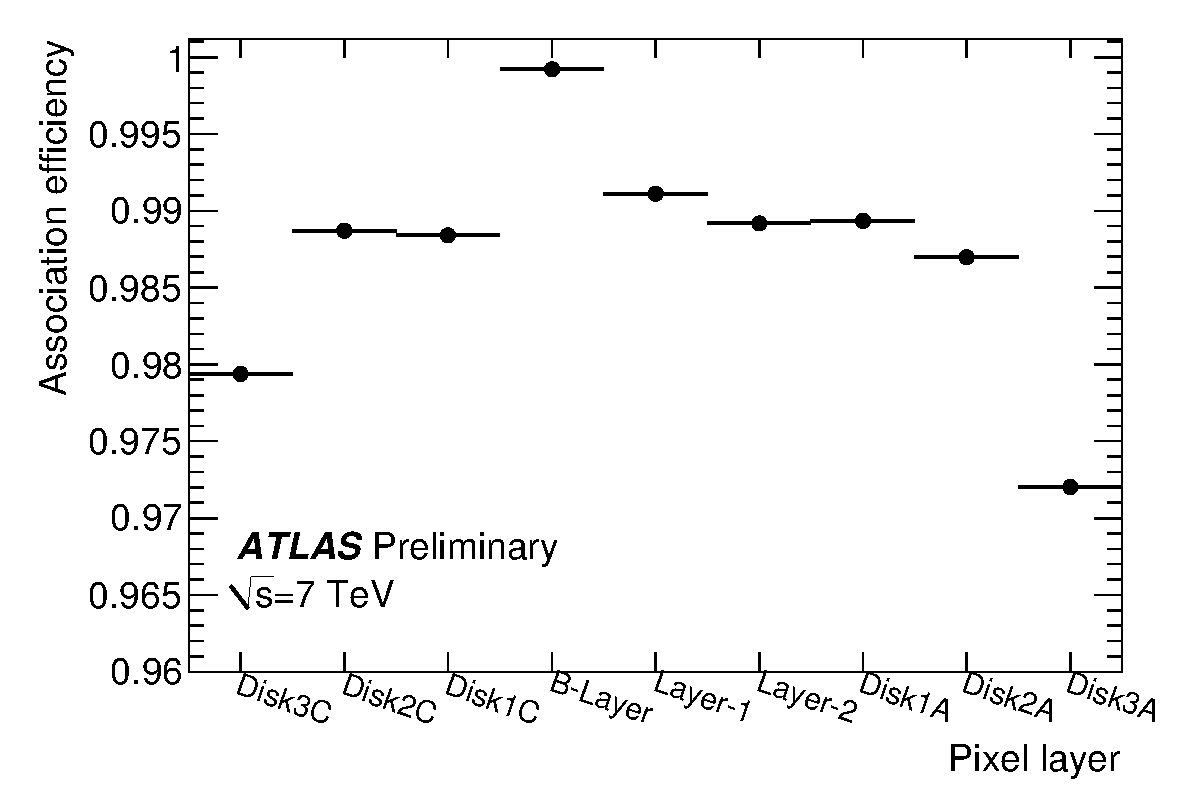
\includegraphics[height=0.33\textwidth]{./figs/Efficiency.pdf}
  \label{sfig:pixelhiteff}
}
\subfloat[Evolution of the module leackage current]{
  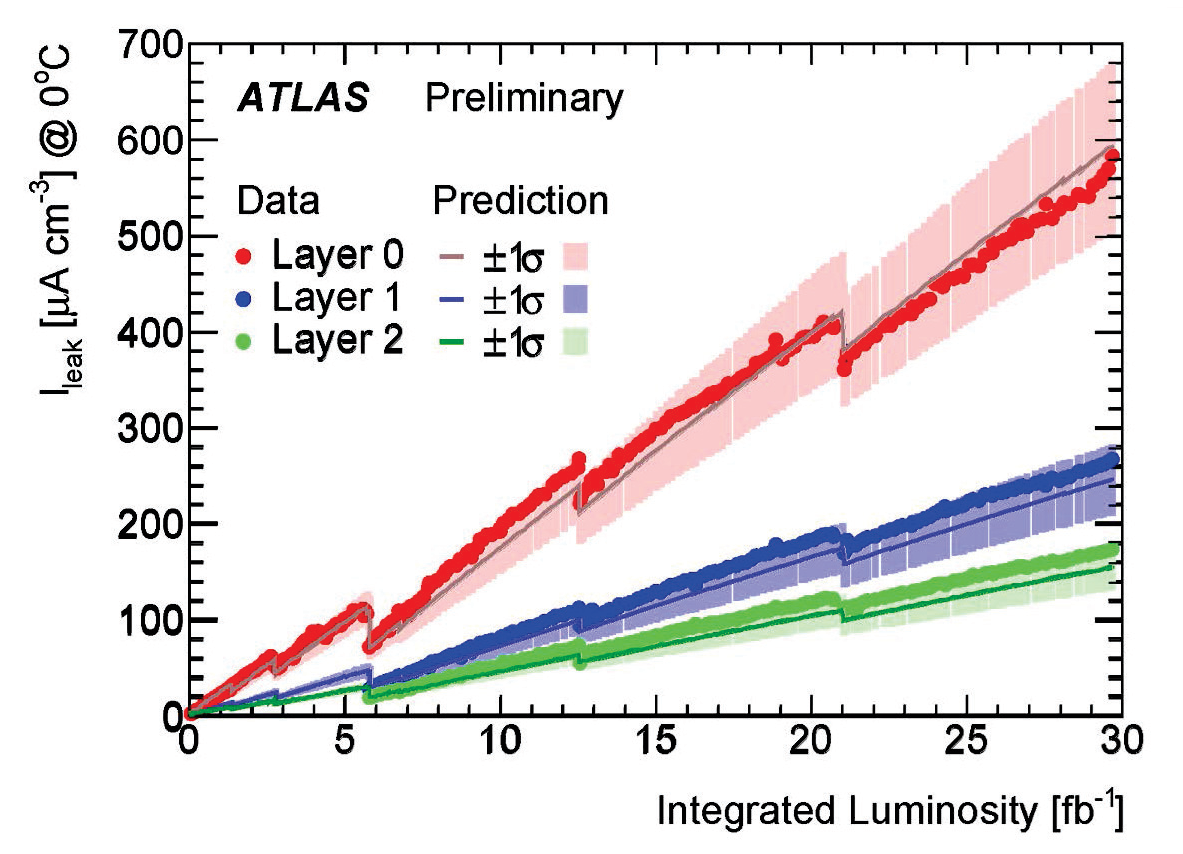
\includegraphics[height=0.33\textwidth]{./figs/hvpp4_CorCur_lumi_Jan2013_total.pdf}
  \label{sfig:leakagecurrent}
}
% \subfloat[Stability of the fitted proton mass]{
%   \includegraphics[height=0.33\textwidth]{./figs/Fitted_Proton_Mass_dEdx.pdf}
%   \label{sfig:pixelprotonmass}
% }
\hfill
\caption[Performance of the pixel detector during \RunOne]{
%
\Fig~\subref{sfig:pixelhiteff} shows the probability for a track to have a hit associated, when passing through a given pixel layer~\cite{Pernegger:1985432}. The uncertainty bars are smaller than the marker sizes. The full efficiency for the \blayer\ is an artefact and stems from the track selection.
% 
\Fig~\subref{sfig:leakagecurrent} shows the average leakage current for the pixel modules as a function of the integrated luminosity during \RunOne~\cite{LaRosa:1956433}.
%
% \fig~\subref{sfig:pixelprotonmass} shows the stability of the fitted proton mass over \RunOne, obtained by inversion of the Bethe--Bloch formula for particle energy loss per depth of material $\mathrm{d}E/\mathrm{d}x$.
}
% \label{fig:DLdataMCcomp7TeV}
\end{figure*}
%%%%%%%%%%%%%%%%%%%%%%%%%%%%%%%%%%%%%%%%%%%%%%%%%%%%%%%%%%%%%%%%%%%%%%%%%%%%%%%






% \subsection{Module recovery and nSQP reconnection}
After the extraction of the pixel package from the \gls{ATLAS} detector, the old \glspl{SQP} were removed and the module failures were ana\-lysed, using a standalone TurboDAQ~\cite{USBPix} setup. 
%
\Fig~\subref*{sfig:disabledmodulesR1} shows the results of the inspection of the 88 faulty modules and predominantly reveals communication faults like unresponsive optoboards and channels or missing detector clock. 
%
The installation of the \gls{nSQP} cured many of the faults outside the active volume due to cabling or broken connections. Nevertheless, sensitive parts of the \glspl{nSQP} introduced new disconnection failures. These could mostly be recovered by careful resoldering, like in the case of the electrical cable feedthrough through the nitrogen isolation end cap. 
%
The high fragility of the detector did not allow to dismount the end caps and barrels, and consequently module or chip related locations could not be accessed and corresponding faults only rarely repaired. Broken \gls{HV} lines, for example, were often not recoverable due to their inaccessible position inside the active detector volume. Exceptions were the recovery of six broken \gls{HV} connections on disk modules using conductive epoxy glue on the module flex. Cable faults in the accessible parts of the \gls{HV} or \gls{DTO} lines directly connected to the active volume could often be fixed by rerouting to alternative lines. The position of the cable failure was determined by \gls{TDR} measurements, making use of the runtime of the signal reflection at the cable discontinuity to infer the spatial distance. This technique has a spatial resolution of about 10~\cm, sufficient to determine the accessibility of the fault. 
%
Alongside the reconnection, all modules and functional detector components underwent a series of tests to verify their functionality before they again became inaccessible, using the \gls{DAQ} and \gls{DCS}~\cite{1748-0221-3-05-P05006}. This process comprised more than 50,000 manual database entries, registering the identification numbers and location of the modules, cables and \glspl{NTC} under test, the \gls{HV}, \gls{LV} line voltage and current values in configured and unconfigured state, results of digital tests and comments on any irregularity. 
%
%
Besides the recovery of modules, together with the installation of the \glspl{nSQP}, additional upgrades were performed. The position of the optoboards, which are sensitive parts of the data transmission, was moved outside the detector volume to ease maintenance. 
%
New optical cables, increasing the number of fibres, were routed from the detector to the counting room, connecting the new optoboards with the \glspl{ROD}. 
%
This will allow to double the data bandwidth of \layerone\ to $160$~Mbps (megabits per second) to cope with the high luminosity expected for \RunTwo. Similarly, the \layertwo\ readout speed is planned to be doubled to $80$~Mbps. These upgrades are planned for the winter shutdowns of 2017 and 2016, respectively.
%
This will be accompanied by renewed back end electronics, using the more peformant new generation of \gls{ROD} and \gls{BOC}, especially developed for \gls{IBL} readout. 




% \subsection{Installation and performance test in the pit}
After the mechanical works and the extensive tests, the pixel detector was lowered into the \gls{ATLAS} experimental cavern and reinserted into the \gls{PST} in a several days operation. Early February 2014, the first modules were reconnected to the \gls{ATLAS} services and the tests, already passed on the surface, were reperformed, to assess possible damage due to the reinsertion. As expected, the highly fragile unpotted \gls{HV} connections suffered the most new failures. After the electrical connections, the cooling lines were closed and tested for leakage under pressure and the new optoboards were installed and connected. The success of the pixel detector refurbishment can be seen in \fig~\subref*{sfig:Pixel_DisableByLayer}, with a significant drop in disabled modules after reinstallation, especially for the crucial \blayer\ (\layerzero). 
%
The works were finished in spring 2014, and the fraction of over 98\% of operative modules is now even higher than at the start of \RunOne. 
%
The \gls{ATLAS} pixel detector will be fully capable of handling the high rates during \RunTwo, once the remaining readout upgrade works have been carried out. 
%
%%%%%%%%%%%%%%%%%%%%%%%%%%%%%%%%%%%%%%%%%%%%%%%%%%%%%%%%%%%%%%%%%%%%%%%%%%%%%%%
\begin{figure*}[tbp!]
\centering
\subfloat[Disabled modules at the end of \RunOne]{
  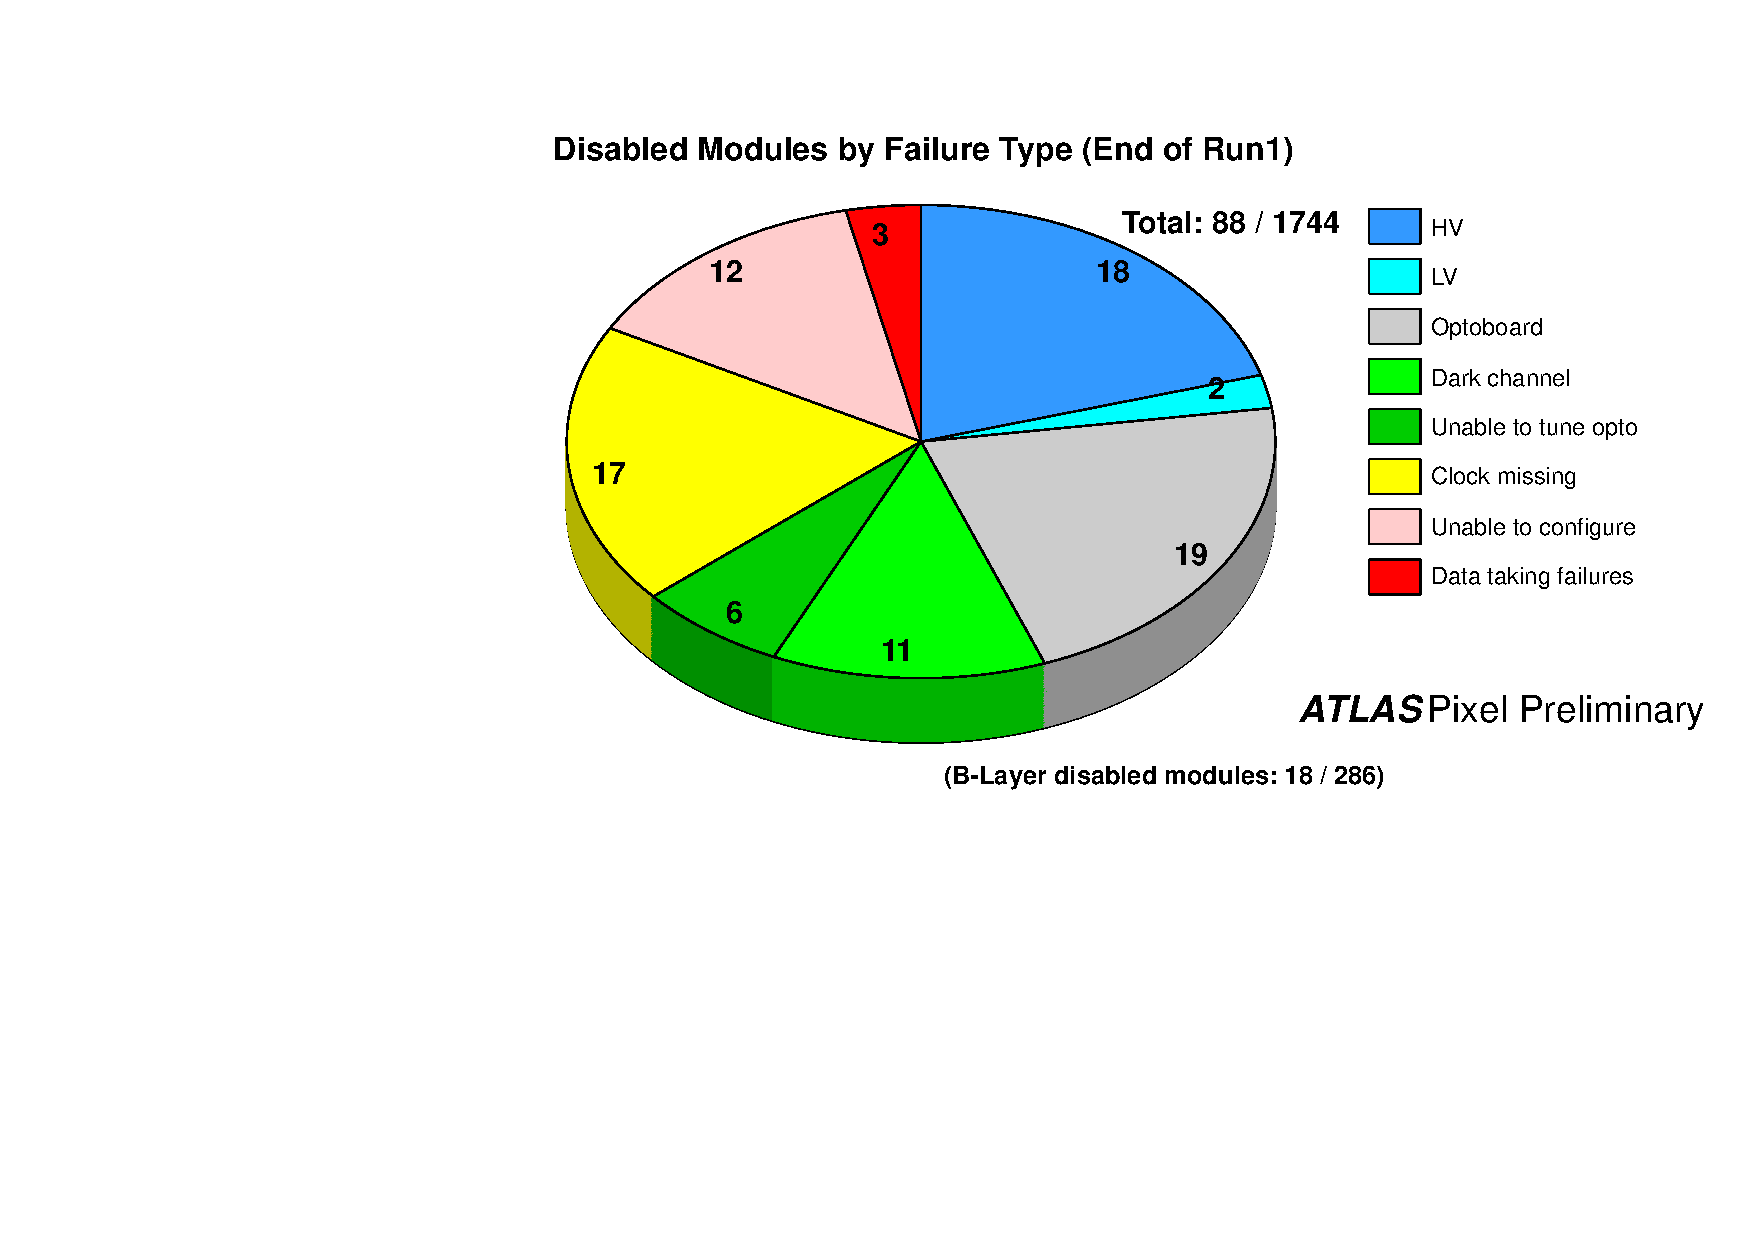
\includegraphics[height=0.33\textwidth]{./figs/EndOfRun1_pixel_failure.pdf}
  \label{sfig:disabledmodulesR1}
}
\hfill
\subfloat[Disabled modules before and after refurbishment]{
  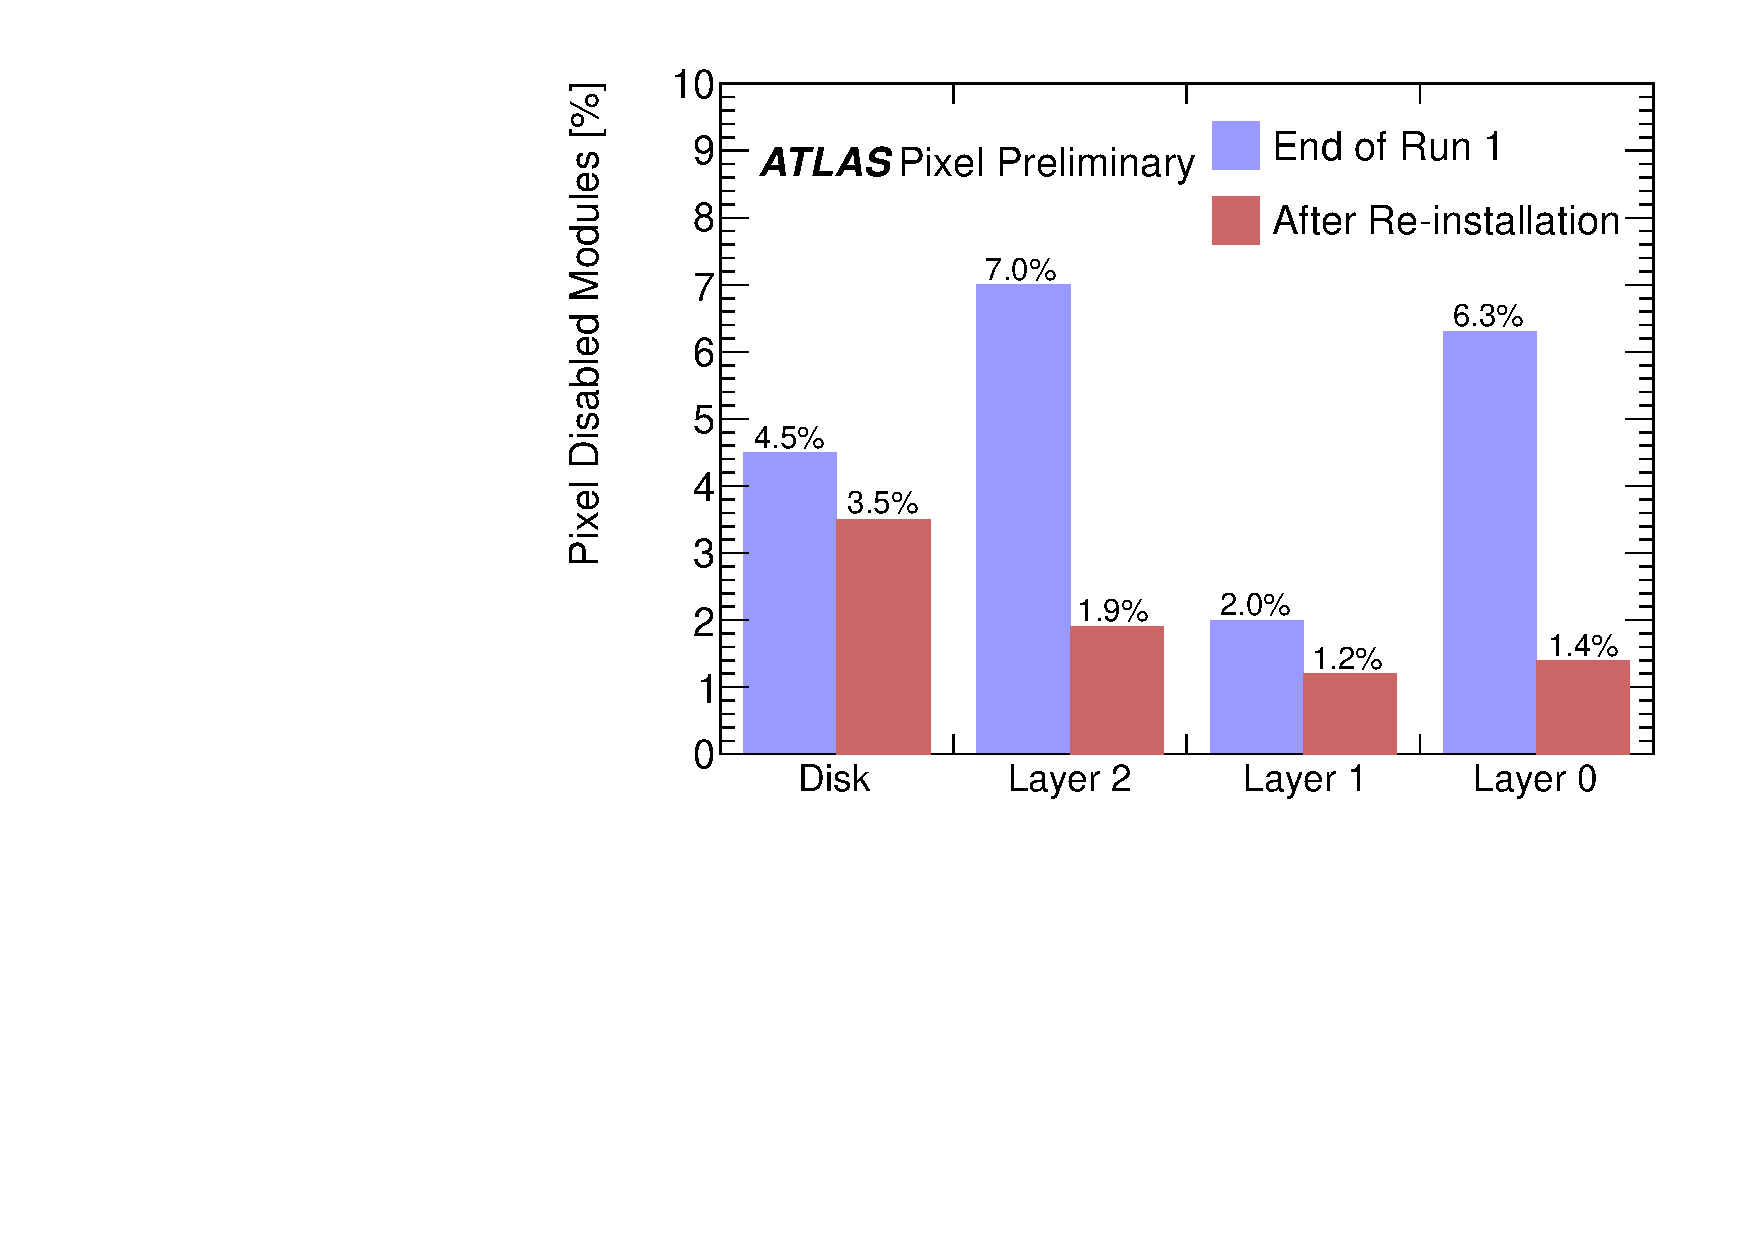
\includegraphics[height=0.32\textwidth]{./figs/Pixel_DisableByLayer.pdf}
  \label{sfig:Pixel_DisableByLayer}
}
\caption[Module failures during the pixel detector refurbishment]{
%
\Fig~\subref{sfig:disabledmodulesR1} shows the number of disabled modules at the end of \RunOne, sorted by failure type.
%
\Fig~\subref{sfig:Pixel_DisableByLayer} shows the number of disabled modules per layer before and after the refurbishment procedure~\cite{ATLASPixelPlots}. 
}
% \label{fig:DLdataMCcomp7TeV}
\end{figure*}
%%%%%%%%%%%%%%%%%%%%%%%%%%%%%%%%%%%%%%%%%%%%%%%%%%%%%%%%%%%%%%%%%%%%%%%%%%%%%%%




















\section{Performance tests of IBL}
\label{sec:IBL}
During \gls{LS1}, the \gls{IBL} detector was assembled at \gls{CERN}. From a total of 20 staves produced, 14 staves were selected, according to a \gls{QA} procedure\cite{ATL-INDET-PUB-2014-006}, including electrical functionality, thermal stress and radioactive source tests. 
%corrosion
During one of the cold electrical tests, a condensation accident occurred, with ice formation on two staves. This lead to a thorough investigation of the damage, during which severe wire bond corrosion was observed. The following inspection of all staves revealed that halogen remnants from the production process acted as catalysts in the presence of water, leading to the corrosion. All staves, produced at that point, were cleaned and reworked, and special care was taken to avoid condensation and humidity at all costs. Once installed at \gls{ATLAS}, the nitrogen atmosphere prevents any further corrosion process and no impact on data taking performance is expected. 
%
The modules of the selected staves can be operated stably at a threshold of 2500~e (elementary charges) and show a noise of 130~e for the planar and 150~e for the 3D modules. This leaves much room to compensate for radiation damage and other degradation effects that might appear during operation with an increased hit threshold. 
%Kerstin sagt, IBL wird bei 2500 und nicht 1500 e betrieben
%
Outperforming the design goal of 1\% by an order of magnitude, a fraction of 0.1\% of dead pixels was reached, with all chips fully operational. 
%
The functionality of the detector was monitored during the module loading on the staves and the assembly of the full \gls{IBL} detector~\cite{BilbaoDeMendizabal:1984087}.
%
The \gls{IBL} was then successfully inserted into the pixel detector in May 2014 and the following \gls{QA} tests confirmed its high performance also after integration into the \gls{ATLAS} systems. 
%bowing
Studies using cosmic rays performed at different temperatures revealed stave deformation of up to 1~\mum\ per K, caused by different thermal expansion coefficients in the support structures. This can be compensated for by taking into account the temperature dependency of the module positions in the detector alignment software. Due to the stability of the stave temperature during a run, this design flaw does not pose a problem for data taking. 
%
In the meantime, the \gls{IBL} has been integrated into the \gls{ATLAS} data taking system and has been operating successfully since the start of \RunTwo. 
%
One of the first cosmic muon events in \RunTwo\ from the end of the year 2014, leaving a track in all four pixel and all four \gls{SCT} layers of \gls{ATLAS}, is shown in \fig~\subref*{sfig:muontrack}~\cite{ATLASRun2EventDisplays}. 
%
With the fourth layer of pixels, the \ljet\ rejection factor of the commonly used \btag\ algorithms will be almost doubled~\cite{IBL-TDR}, as shown in \fig~\subref{sfig:lightrejectionIBL}. This will be a huge benefit for precision measurements in \RunTwo. 
%
%%%%%%%%%%%%%%%%%%%%%%%%%%%%%%%%%%%%%%%%%%%%%%%%%%%%%%%%%%%%%%%%%%%%%%%%%%%%%%%
\begin{figure*}[tbp!]
\centering
\subfloat[First cosmic muon event in the ID]{
  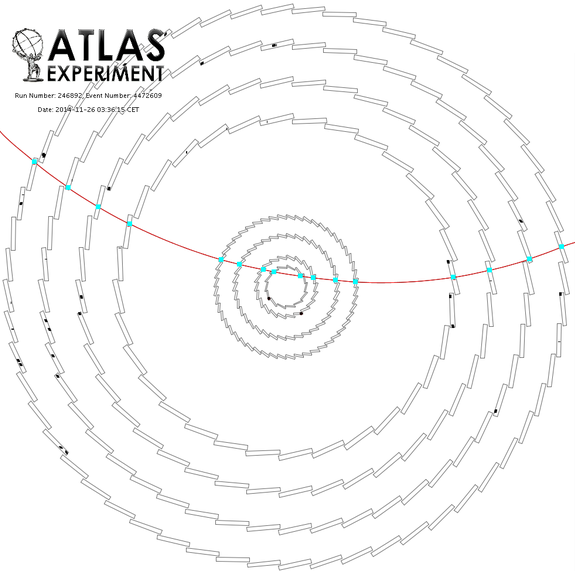
\includegraphics[height=0.44\textwidth]{./figs/IBL_cosmic_ray_inverted_cropped.png}
  \label{sfig:muontrack}
}
\hfill
\subfloat[\Ljet\ rejection factor with and without the IBL]{
  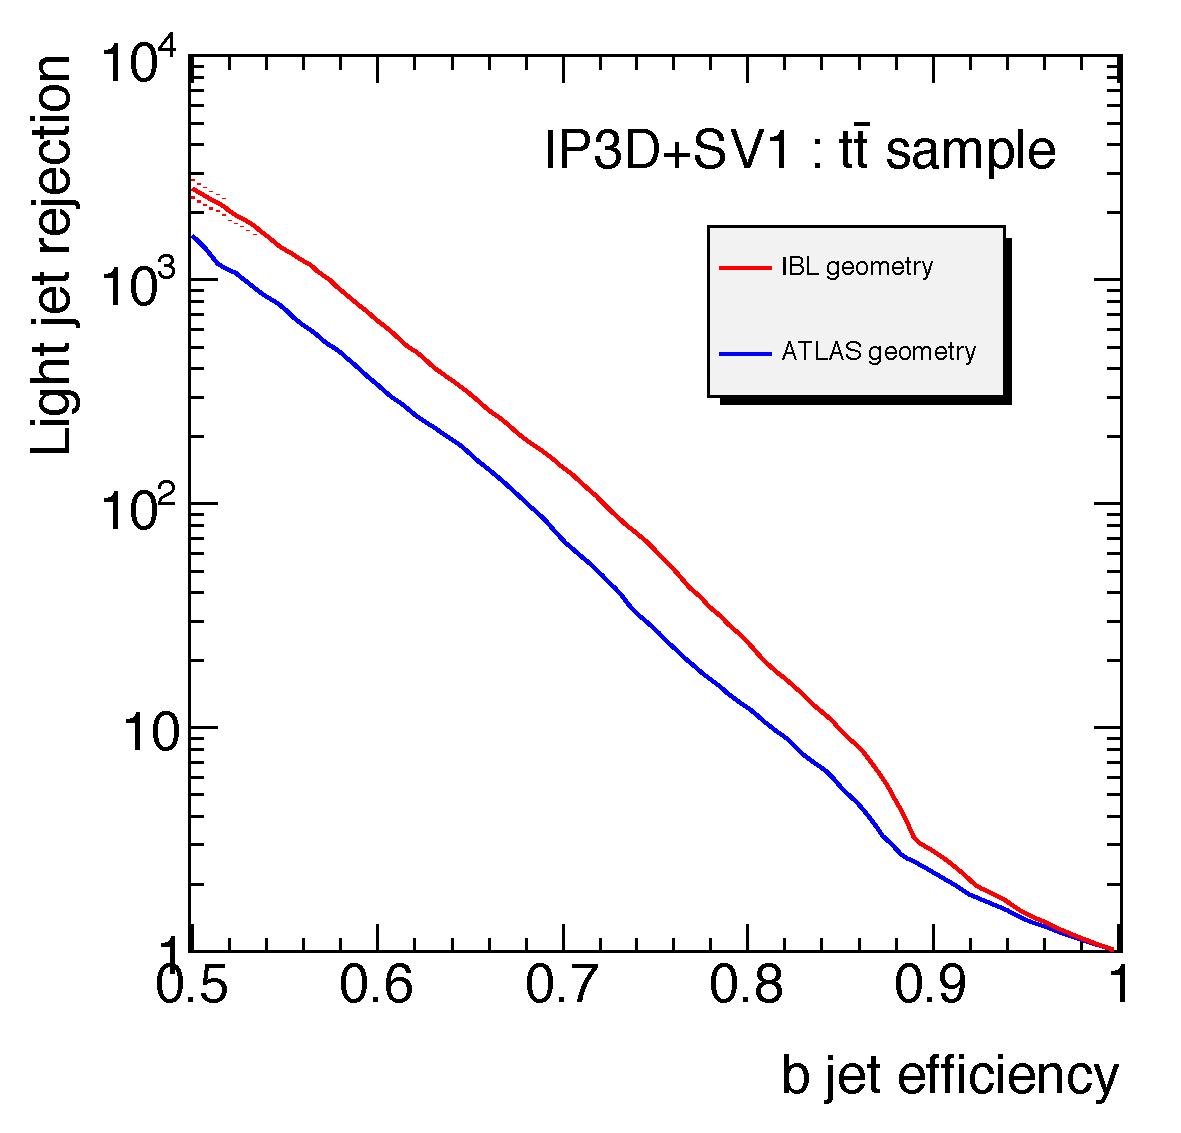
\includegraphics[height=0.44\textwidth]{./figs/IBL_lightrej_factor.pdf}
  \label{sfig:lightrejectionIBL}
}
\caption[Performance of the upgraded pixel detector]{
%
\Fig~\subref{sfig:muontrack} shows one of the first cosmic muon events leaving a track in all four layers of both the new pixel detector including \gls{IBL} and the \gls{SCT}~\cite{ATLASRun2EventDisplays}. 
%
\Fig~\subref{sfig:lightrejectionIBL} shows the \ljet\ rejection factor as a function of the \btag\ efficiency evaluated for the \btag\ algorithm IP3D+SV1 on a \ttbar\ \gls{MC} sample for \gls{ATLAS} with and without the \gls{IBL}~\cite{IBL-TDR}. 
}
\label{fig:IBLsuccess}
\end{figure*}
%%%%%%%%%%%%%%%%%%%%%%%%%%%%%%%%%%%%%%%%%%%%%%%%%%%%%%%%%%%%%%%%%%%%%%%%%%%%%%%







\section{Summary}
\gls{LS1} has been used to prepare the \gls{ATLAS} \gls{ID} for the challenges of \RunTwo. The previous pixel detector has been refurbished and an additional innermost layer of pixel modules, \gls{IBL}, has been inserted. The pixel detector is now in excellent condition and is expected to continue reliable operation throughout \RunTwo, until it will eventually be fully replaced for the conditions of \gls{HLLHC} in 2024.
%
The pixel detector is operating successfully and the new \gls{IBL} detector contributes to the excellent \btag\ performance during \RunTwo.